\documentclass[a4paper,10pt]{article}
\usepackage[utf8]{inputenc}%PAQUETE PARA CORRECCION DE TIPOGRAFIA PARA ESPAÑOL
\usepackage[english,spanish]{babel}%PAQUETE DICCIONARIO ESPAÑOL
\usepackage{amssymb}%PAQUETES COMPLEMENTO PARA TIPOGRAFIA MATEMATICA
\usepackage[pdftex]{graphicx}%PAQUETE PARA LA INCLUSION DE IMAGENES jpg, png Y pdf
\usepackage{pdfpages}
\renewcommand{\rmdefault}{phv} % Arial
\renewcommand{\sfdefault}{phv} % Arial
\author{Dini, A. \\García Blesa, M.}%AUTOR DEL DOCUMENTO
\date{\today}%FECHA DE EDICION DEL DOCUMENTO
\title{
\includegraphics[scale=0.5]{img/nPyLogo.pdf}\\\textbf{Nuclear Py}}%TITULO DEL DOCUMENTO

\begin{document}
\selectlanguage{english}
\maketitle

\begin{abstract}
nPy is a configurable graphical interface (GUI) written in Python 2.7 and PyQt4. It has been built as a new graphical platform to run applications used in nuclear technology in a friendly fashion. Usually such programmes run from a terminal and require very specific and long string parameters. nPy enables the addition of any program or command into its menu and launch it subsequently, capturing the standard output produced and showing it on the main screen. A special Sequence Table tool allows the user to edit any list of system processes –one after the other– with or without parameters, editing at the same time the main graphic menu and running that list with a simple click.
\end{abstract}
\newpage

\tableofcontents
\newpage

\section{Introduction}

nPy is a configurable graphic interface written in Python 2.7 and PyQt4 that enables the addition of any program or command into its menu and launching it subsequently, showing the standard output produced on the main screen.

The aim of the project is to build a graphical environment to design any complex sequence of processes, and launch it as a list, enabling the change of any parameter for each system command or program.

nPy provides a graphical solution. A dynamic table application will allow the user to create any list of processes, defining their order and parameters, enabling the edition and deletion of rows as needed.

It is possible to launch nPy in almost every operating system. It has been tested in Windows 8 and windows 10, and linux Ubuntu 18.04, linux Mint 17.2, linux Debian 8.x, even Raspbian for Raspberry Pi and others.

\subsection{nPy Elements}

At the beginning nPy presents a main window divided into two sections: a tree view and a tab section.

The tree view is a conventional application. It allows the user to
navigate through the directories, and open a text file in the embedded
text editor application.

\begin{center}
 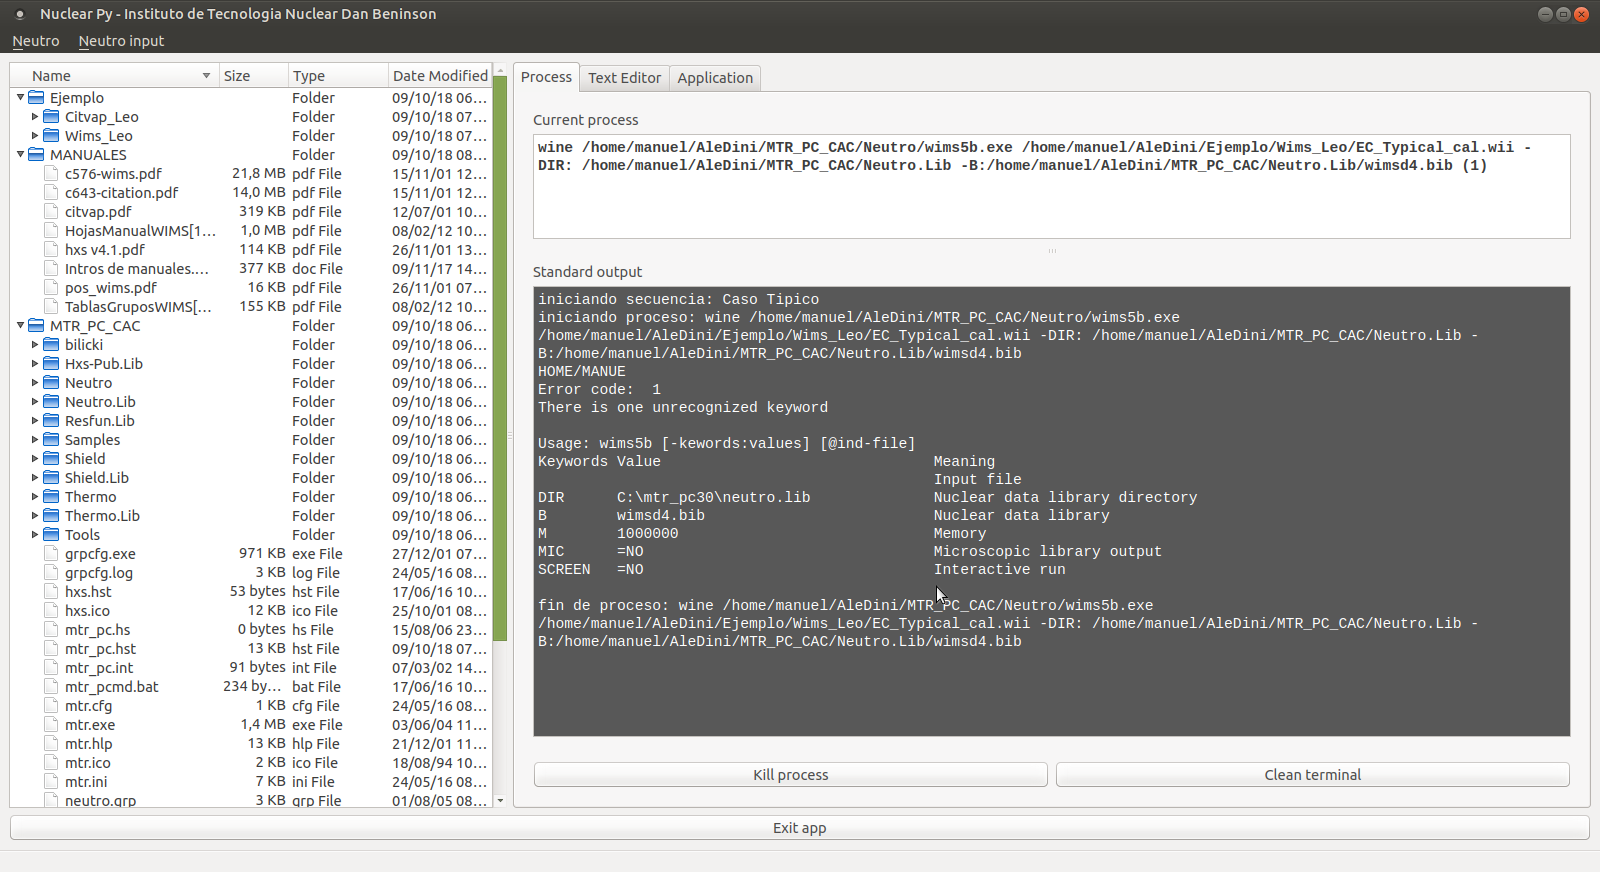
\includegraphics[width=\textwidth]{img/mainWindow.png}
\end{center}

\noindent The tab section includes three applications:

\begin{itemize}
 \item Process
 \item Text editor
 \item Configuration
\end{itemize}

\subsection{Process}
This tab shows two fields configured as outputs. The Current Process indicates which process of the list is running. The Standard Output shows the process in real time as shown in a regular system terminal.

It is possible to stop any process at any time and continue with the next in the list using the Kill process button, as well as to clean the terminal to start a new list of process by pressing the Clean terminal button.

\subsection{Text Editor}

A flexible environment was provided to enable the execution of complex command lists with any parameters. 

\begin{center}
 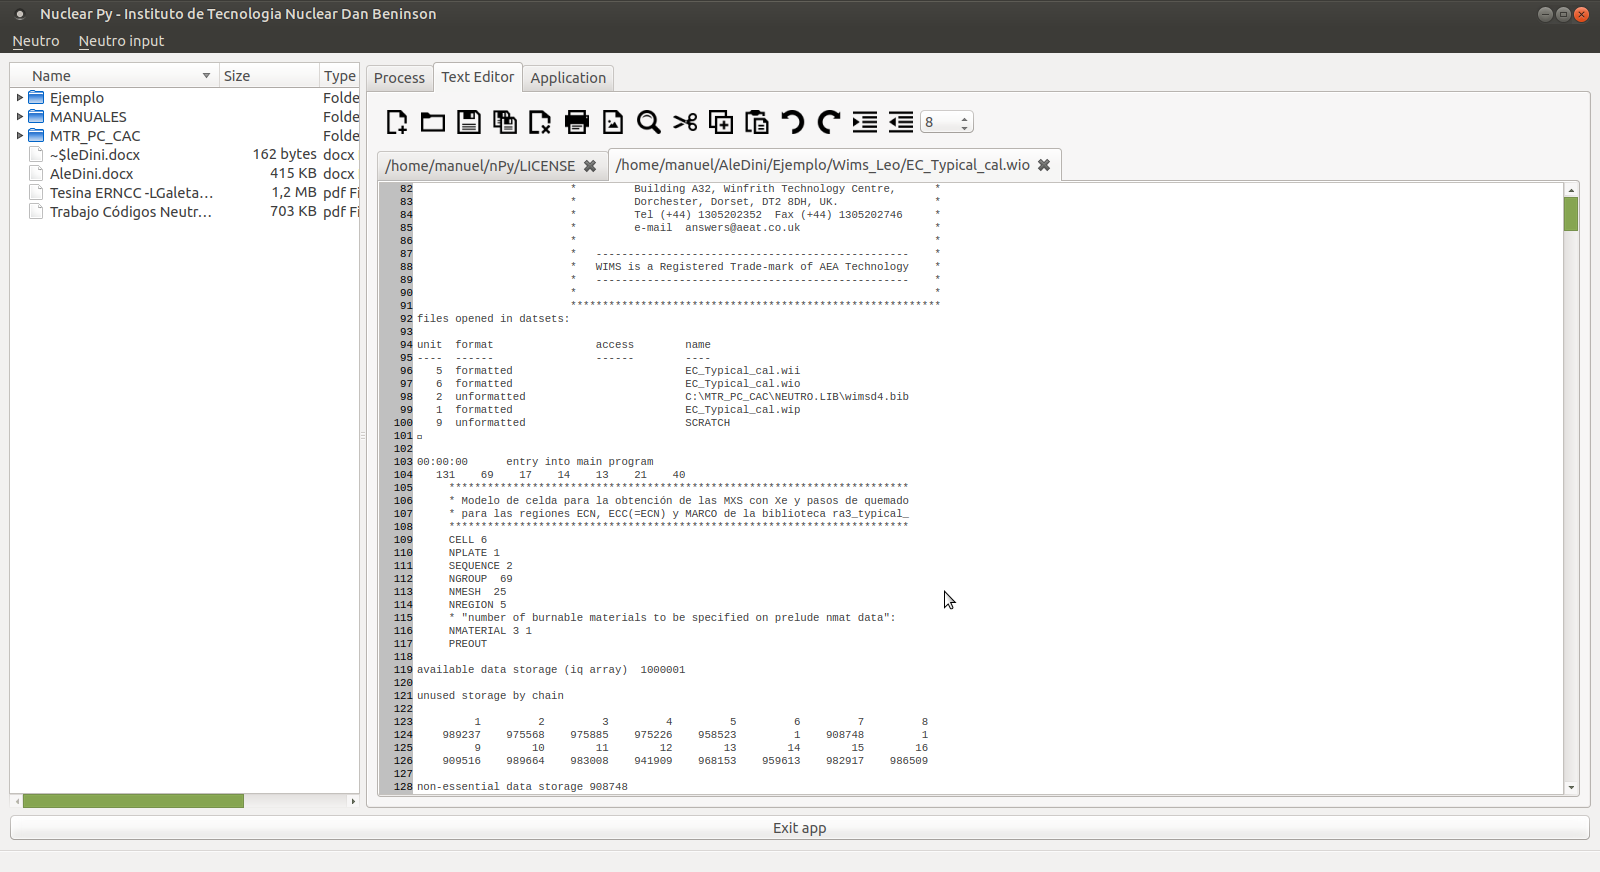
\includegraphics[width=\textwidth]{img/textEditor.png}
\end{center}

For such purpose a simple but powerful text editor was included. It works as an assistant to view and edit the in-files and out-files in every process defined. This embedded text editor was conceived as a special programming application with a highlighted font.

It supports python syntax highlighting and multiple tabs, so you can edit your files without needing anything else.

\subsection{Application}

The third tab is a special section which, in turn, presents two tabs: Sequence Table and Environment.

The first of these two tabs, the Sequence Table, shows the sequence table application which helps the user to set the list of processes.

The second tab, Environment, allows the user to change the root path and the initial path required to set the initial position in the tree view application.

\begin{itemize}
 \item Home
 \item Process Tab
 \item Squence Table User manual
 \item Text-Code editor
\end{itemize}

\section{Install Guide}

\subsection{General considerations}

You can download \textbf{nPy} from github: 
\begin{verbatim}
 https://github.com/alete89/nPy/releases
\end{verbatim}

nPy runs over Windows and Linux operative systems (OS). To complete the installation is needed to follow instructions depending on the OS in use. nPy needs Python 2.7 and PyQT4 framework to run. All those are free software and can be downloaded from every respective official site.
\bigskip 

\noindent Last Python release: 
\begin{verbatim}
https://www.python.org/download/releases/2.7/
\end{verbatim}

\noindent Last PyQT4 release: \begin{verbatim}    
https://www.riverbankcomputing.com/software/pyqt/download
\end{verbatim}
  
\subsection{On Linux system}

Almost every linux system comes with python 2.7 preinstalled. In other case you can install it using a system terminal:
\begin{verbatim}
apt-get install python2.7
\end{verbatim}

\noindent PyQT4 usually doesn't comes preinstalled so we must to install. We can use the same way before:
\begin{verbatim}
apt-get install python-pyqt4 
\end{verbatim}

\noindent A compact way to install both at the same time:
\begin{verbatim}
apt-get install python2.7 python-pyqt4 
\end{verbatim}

\subsection{On Windows System}

Usually windows doesn't comes with python preinstalled. So you need to download it from the official site and run the simple install.

The same occurs with the PyQT4 libraries. You can download it from 
\begin{verbatim}
https://riverbankcomputing.com/software/pyqt/download 
\end{verbatim}
\noindent and run the windows installer.

\subsection{Pip (Python Package Index)}

Optionally pip to install the packages. Pip is a dedicated python package system to get python libraries and others you can use to install all python's needs to run nPy. It is simple to use. Just run in a system terminal as follows:

\begin{verbatim}
 pip install python2.7 pyqt4
\end{verbatim}

\noindent Under Windows systems, pip wont find PyQt4 to install, .whl are provided here: 

\begin{verbatim}
https://www.lfd.uci.edu/~gohlke/pythonlibs/#pyqt4 
\end{verbatim}

\section{Process Tab}

The first screen that you see when you run nPy is the Process tab.

\begin{center}
 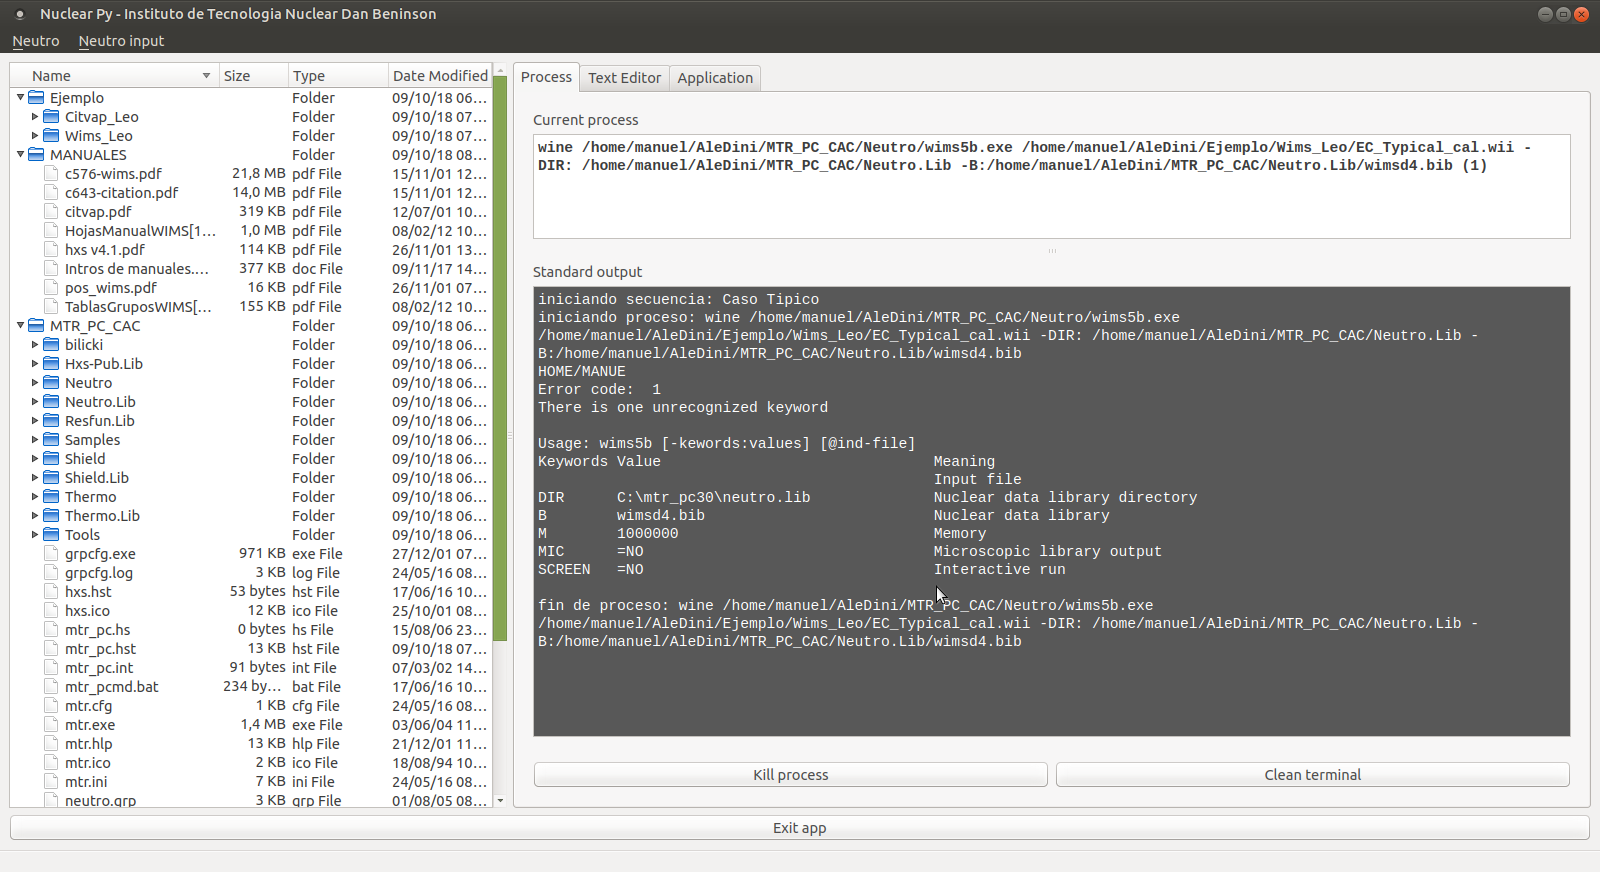
\includegraphics[width=\textwidth]{img/mainWindow.png}
\end{center}

On the left side of the screen you have a TreeView that is visible for all the screens, enabling to browse your file system. The main tab features two outputs. Current process (experimental) shows the sequence of commands as they are being executed. Standard output shows exactly the output of every command executed by nPy.

If, eventually, a command running is required to stop, you can press the Kill process in order to terminate its execution.

Clean terminal button just clears the Standard output box.

\section{Running nPy}

\subsection{on Linux}

Unpack the nPy.tar. Open a terminal, place in the nPy directory and simply run
\begin{verbatim}
python nPy.py 
\end{verbatim}

\subsection{Running on Windows}

Just excecute the nPy.exe

\section{Sequence Table}

\subsection{nPy Sequence Table (ST)}

The ST represents the core of the nPy application. The table structure is a simple way to store information needed to configure system processes (i. e.  it is possible to order any process that you wish to run on a terminal) as well as to configure information to create a graphical menu.

The purpose of its editing table is to solve three different problems: the first one is to create a complex process sequence to be run orderly, with no limit to the number of parameters defined. The second one is to create graphical options in the main menu, and the third one is to make it friendly and simple.

The aim of it is to configure different processes needed, including any parameters for each one, and run all of them one after the other, with a single click. The correct configuration will create a button in the main menu, and a context menu for each parameter set in the table.

\subsection{Sequence table: Properties}
This table has been designed with 7 columns:

\begin{itemize}
    \item \textbf{id}: simple auto numeric id
    \item \textbf{Menu}: is the first level name menu, is a string value
    \item \textbf{Submenu}: is the second level name menu (sub menu), is a string value
    \item \textbf{MenuPosition}: indicates the sub menu position, is a integer value
    \item \textbf{Order}: indicates the order of this process in the list, is a integer value
    \item \textbf{Command}: the system command will run, is a string value
    \item \textbf{Loop:} to set how many times to run a process before to the next in the list, is an integer value
\end{itemize}

In the ST application, each process must be defined in one row. So, we define a list of processes in ST. We number them, and execute them in ascending order.

\subsection{Command String Syntax}

As simple as it looks, it is possible to fill every gap in the command column. You can run a simple system command by filling the cell. You can also run a complex command using parameters, exactly in the same way you do it in a regular system terminal.

\begin{center}
 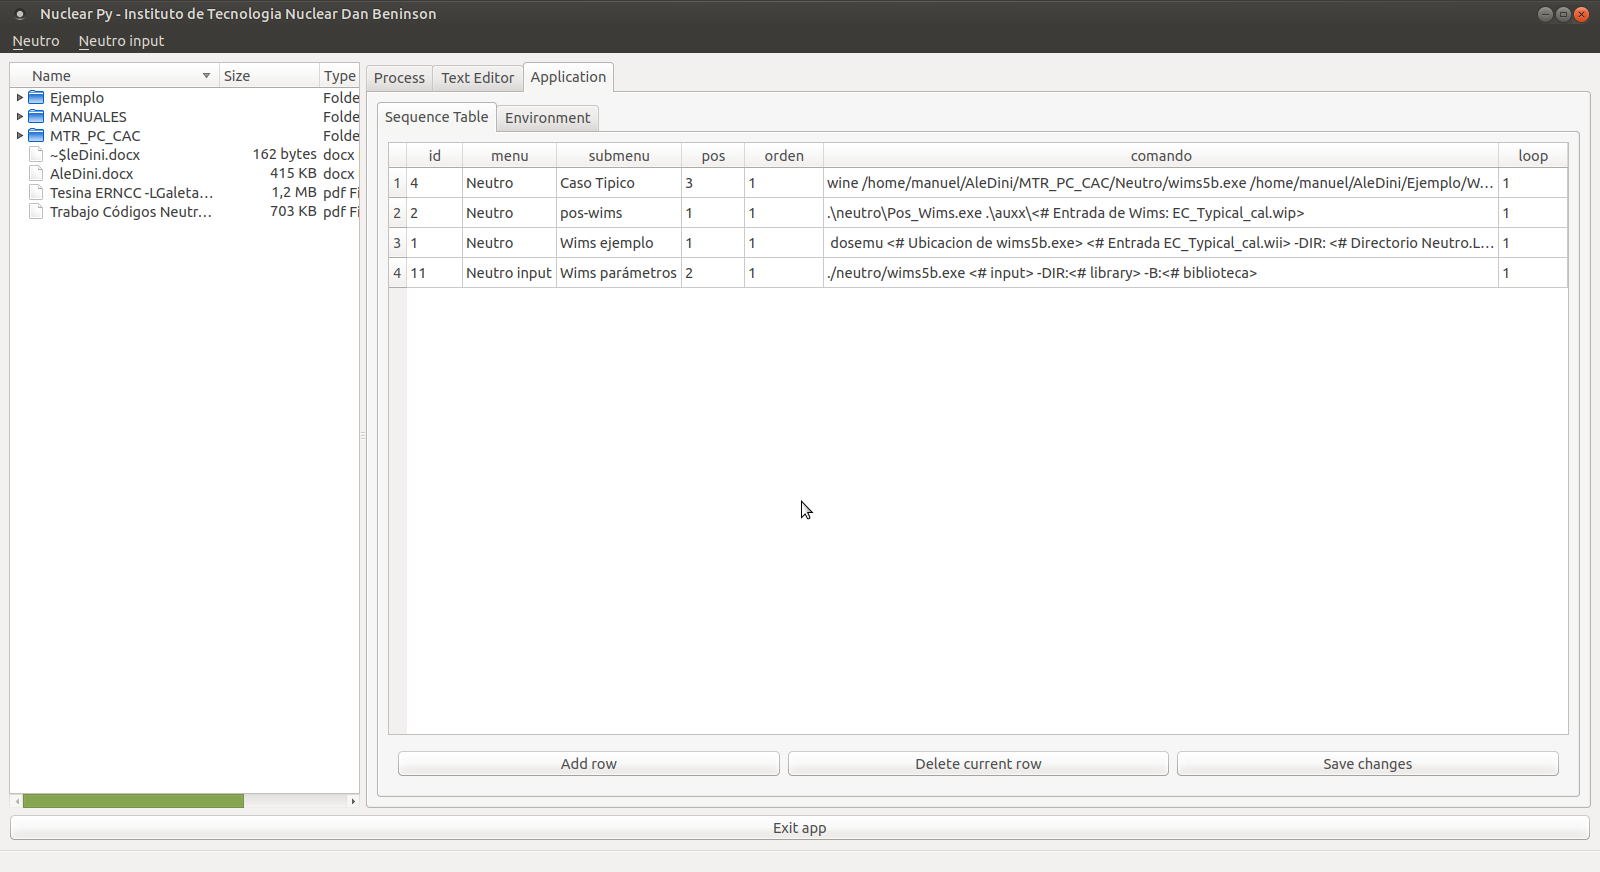
\includegraphics[width=\textwidth]{img/sequenceTable.png}
\end{center}

It is possible to create a context menu to set any different parameters quickly for any command. To write a correct row in the ST a simple syntax rule is required to define the string in the command column in order to create a useful context menu properly. A typical running command presents a very simple structure in a system terminal. Usually we write commands in it as follows:

\begin{verbatim}
user@I7-system ~ $ program [parameter 1] [parameter 2] 
... [parameter n]
\end{verbatim}

In the \textbf{Command} field (in our ST) the syntax is very similar with a small difference: write $< >$ instead $[]$, and describe the parameter between them. Finally the command must be written as follows:

\begin{verbatim}
program <explanation for parameter 1> <explanation for parameter 2> 
... 
<explanation for parameter n>
 \end{verbatim}

The string between the $< >$ will be shown in the graphic context menu as a short message, in a built dynamic form: 
\begin{center}
 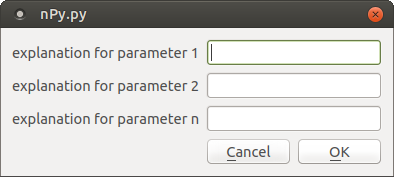
\includegraphics[width=\textwidth]{img/contextMenuExampleString.png}
\end{center}

\bigskip 

After those settings, nPy will be ready to launch lists of programs, commands, scripts, and so on. Anything you can launch from a terminal.

\bigskip 

\noindent As an example you can write on the ST:
\begin{verbatim}
 dosemu <Ubicacion de wims5b.exe> <Entrada EC_Typical_cal.wii> 
 -DIR: <Directorio Neutro.Lib> -B:<Biblioteca wimsd4.bib>
 \end{verbatim}
 
 \noindent and nPy will show the next context menu:
\begin{center}
 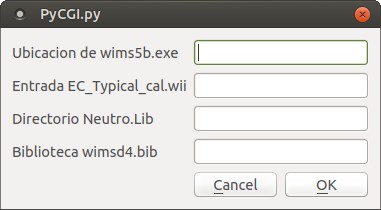
\includegraphics[width=\textwidth]{img/contextMenuString.png}
\end{center}

\bigskip 

It is often needed to pick a file (ussually the file path) to select it as a parameter. This is possible to set in nPy to get a graphic menu for a selection file. Simply write $\#$ as the first character after $<$, as follows: 

\begin{verbatim}
program <# Select file 1> <# Select file 2> ... <# Select file n>
 \end{verbatim}

Thus nPy will create a dynamic menu to select a file into the system for each $<\# ...>$ found on the 
string.

\begin{center}
 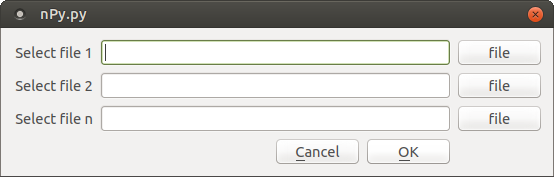
\includegraphics[width=\textwidth]{img/contextMenuExampleFile.png}
\end{center}

\noindent An example:

\begin{verbatim}
 dosemu <# Ubicacion de wims5b.exe> <# Entrada EC_Typical_cal.wii> 
 -DIR: <# Directorio Neutro.Lib> -B:<# Biblioteca wimsd4.bib>
 \end{verbatim}

\begin{center}
 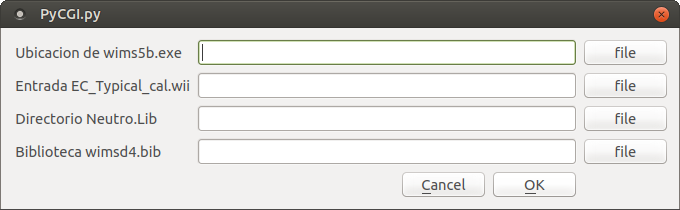
\includegraphics[width=\textwidth]{img/contextMenuFile.png}
\end{center}

\noindent Is possible to combine both techniques as is needed:

\begin{verbatim}
program <# Select file 1> <explanation for parameter 1>
 \end{verbatim}

 \begin{center}
 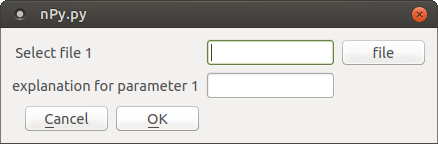
\includegraphics[width=\textwidth]{img/contextMenuExampleCombined.png}
\end{center}

\noindent An example:

\begin{verbatim}
 dosemu <Ubicacion de wims5b.exe> <# Entrada EC_Typical_cal.wii> 
 -DIR: <# Directorio Neutro.Lib> -B:<Biblioteca wimsd4.bib>
 \end{verbatim}

\begin{center}
 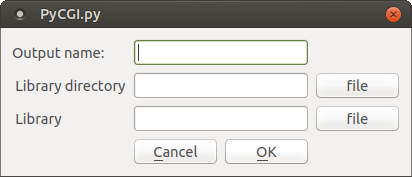
\includegraphics[width=\textwidth]{img/contextMenuCombined.png}
\end{center}

\subsection{Create a Sequence of Processes}

Knowing how to write a single process, will create a sequence putting those in order. An example will be any good to start an explanation. 

\begin{center}
 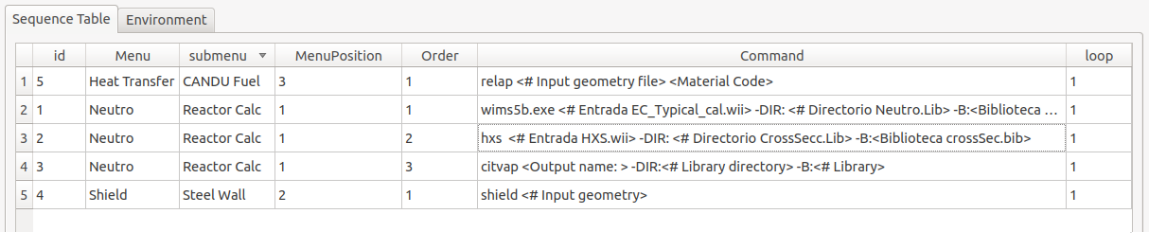
\includegraphics[width=\textwidth]{img/orderingSequence.png}
\end{center}

In the following configuration has been defined three processes: two single processes (\textbf{CANDU Fuel} and \textbf{Steel Wall}) and one sequence of processes (\textbf{Reactor Calc}).

Is simple as define the ``Order'' as follows in the same place in the menu:

\begin{center}
 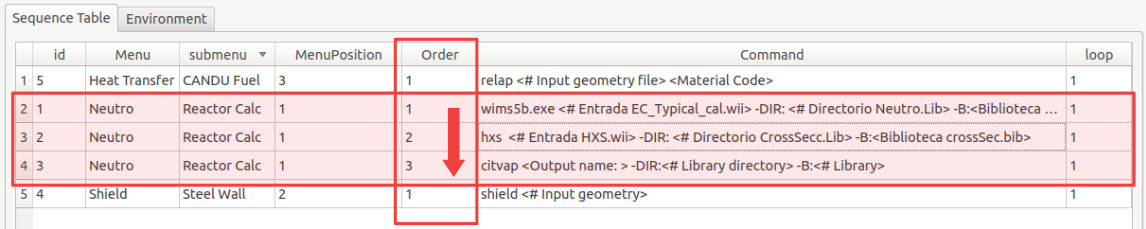
\includegraphics[width=\textwidth]{img/orderingSequenceMark.png}
\end{center}

nPy will create a context menu with all options setted at ST.

\begin{center}
 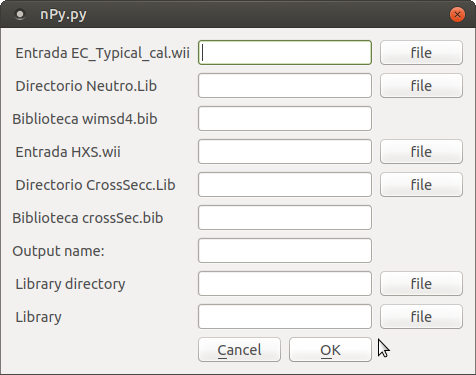
\includegraphics[width=\textwidth]{img/orderingSequenceContextMenu.png}
\end{center}

\subsection{Setting and ordering the main menu}

It is possible to configure the main menu by arbitrarily filling correctly the columns menu, submenu, submenu position and sequence order.

If we consider a menu and its submenus as a set and subset system, we can order the information as levels. nPy has been created to configure the information up to a second level (being the context menu the third level).

The menu column is a string type value, and will show the text at the front of the main menu. This is the first level.

A second level is given by the values submenu and submenu position: submenu is a string type value and its button will be shown inside the first level. Its corresponding submenu position indicates the position in that menu and it is identified with an integer value.

\subsubsection{A Simple Example}

The next example will create two buttons in the main menu: Draw program and Example Menu. Inside the Example Menu option, the user will find three buttons: Sequence test, Python parameters test and Python GPS.

Inside the Sequence test submenu nPy three processes will run ordered by the submenu position.

\begin{verbatim}
id;menu;submenu;posicion en menu;orden en secuencia;comando;loop 
1;Draw program;gimp;1;1;gimp;1 2;Example Menu;Sequence test;1;
2;python /home/alete/git/PyCGI/scripts/simple_print.py;1 
3;Example Menu;Sequence test;2;3;python ./scripts/print_loop.py;1 
4;Example Menu;Sequence test;3;4;python ./scripts/donde.py;1 
5;Example Menu;Python parameters test;2;1;python ./scripts/
parameters.py <un param><otro param>;1 
6;Example Menu;Python GPS;4;1;python ../../Desktop/donde.py;1
\end{verbatim}

\noindent Finally, there is no limit defined to add files to the ST.

\subsection{ST and the Main Menu}

When a process is set in the ST, one button is added in the main menu. If the command in a row is a simple system command or program, nPy will launch it immediately and will show the standard output. If the command has been set with parameters, nPy will create a context menu before launching.

In the process tab, nPy shows two fields: Current Process and Standard Output. The first one shows the current process in the list contained in ST. The second one is the standard output for each process in the list.

It is possible to stop any process and to continue with the next, using the kill process button.

\subsection{A single execution process}

A list of processes will be executed in order, one after the other. This has an important implication: nPy cannot launch more than one process in the ST at a time. This characteristic has been chosen by design in order to guarantee that nPy -as a launcher program- does not modify or interfere with anything during a current process run.

A single execution program will create a simple button with no context menu. It means that the sequence will start immediately showing the output.

\subsection{The Standard Output}

nPy will show the standard output for the current process, the one that is running. When a process listed ends and the next one continues, nPy will notify it to the user and will start to send the new current process to the standard output.

It is possible to view the whole output as a text field. Consequently, it is possible to copy and edit it using the text editor. Frequently it is necessary to know the complete output. nPy provides a simple solution by putting all the outputs in sequence, one after the other.

\subsection{Customizing}

\subsection{Customizing the ST}

The ST application writes a simple .csv file saved in the nPy main directory. If it is necessary to change the settings for a complete different list of processes, it can be done beforehand and switch the .csv files, one by one.

\begin{center}
 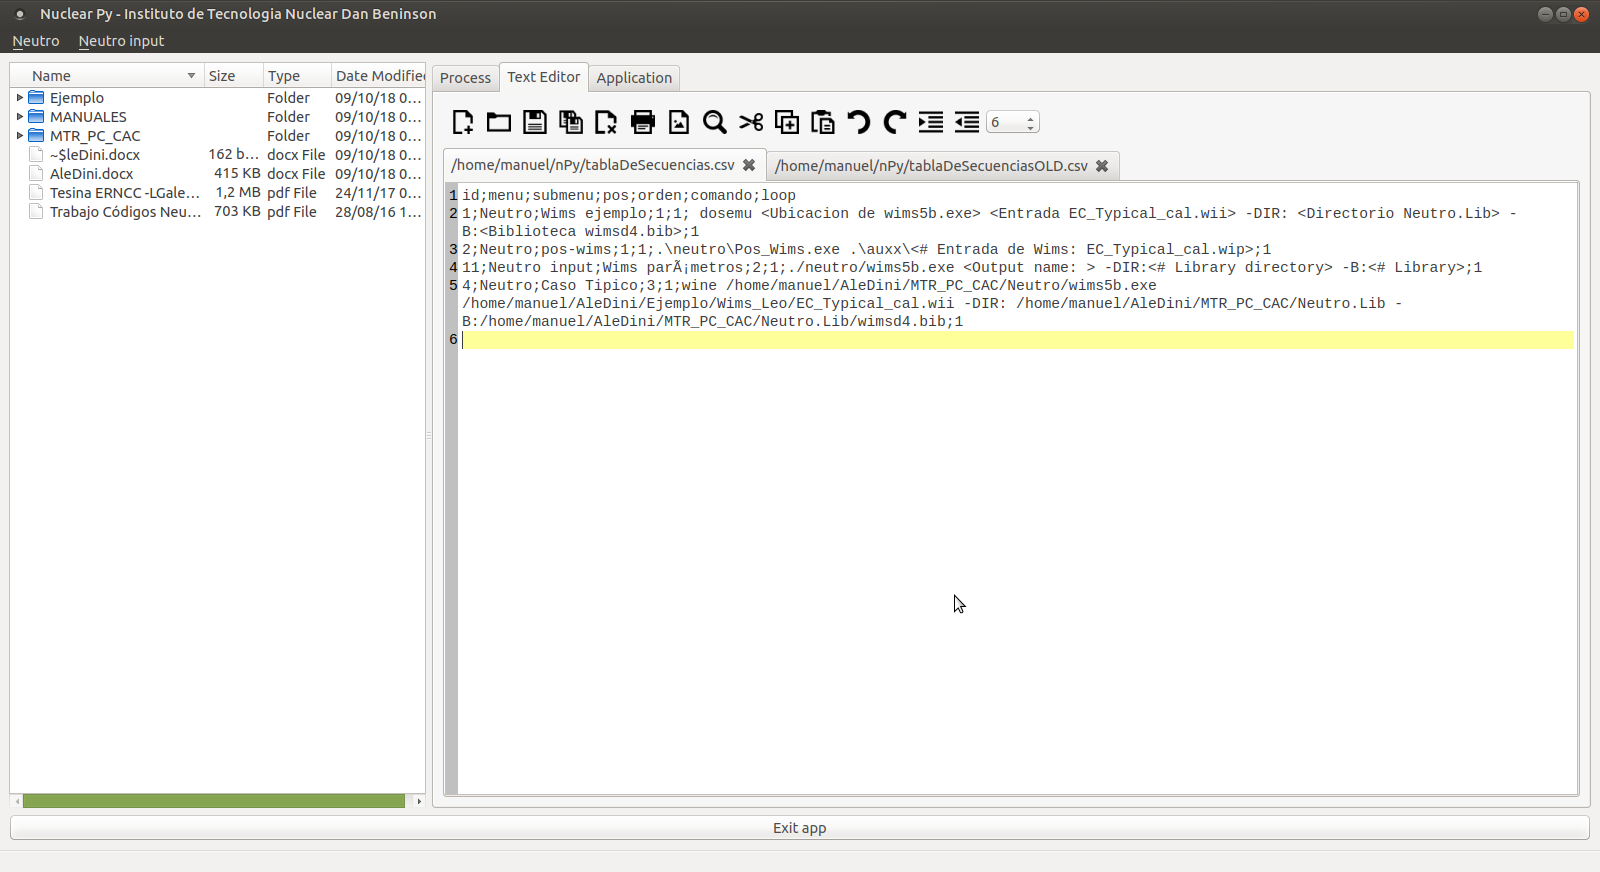
\includegraphics[width=\textwidth]{img/tablaDeSecuenciasConfig.png}
\end{center}

As shown in the picture, it is possible to edit a new ST by hand if the user knows exactly what he/she wants.

\subsection{Customizing directories}

It is possible to set the work directory and the tree-view directory at the Environment tab.

 \begin{center}
 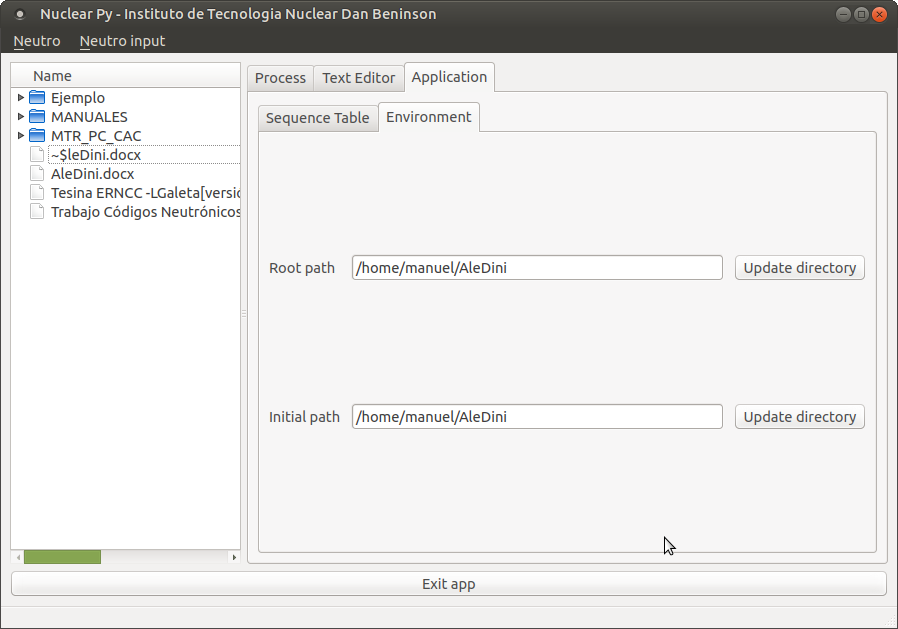
\includegraphics[width=\textwidth]{img/environment.png}
\end{center}

The \textbf{root path} sets the main location where the system starts to run by default, and the initial path sets the initial view location for the tree-view application.

\section{Windows Build}

You can always run nPy through python nPy.py either in windows or linux systems. We also provide windows .exe binares, that can be made following the next steps under a linux system:

\subsection{Install wine, and Python under wine.}
\begin{verbatim}
sudo apt install wine

wine msiexec /i python-2.7.15.msi /L*v log.txt
\end{verbatim}

\noindent you may download latest Python 2.7 release from python web site.

\subsection{Install PyInstaller on wine}
\begin{verbatim}
cd ~/.wine/drive_c/Python27 
\end{verbatim}

\subsection{Install PyQt4 on wine}

\noindent Get .whl from here (https://www.lfd.uci.edu/~gohlke/pythonlibs/\#pyqt4) move it to: 
\begin{verbatim}
cd ~/.wine/drive_c/Python27

wine python.exe Scripts/pip.exe install PyQt4-4.11.4-cp27-cp27m-win32.whl
\end{verbatim}

\subsection{Build.exe}
\noindent cd into nPy folder 

\begin{verbatim}
 wine ~/.wine/drive_c/Python27/Scripts/pyinstaller.exe --onefile -p 
 "C:\Python27\Lib\site-packages\PyQt4" nPy.py
\end{verbatim}

\noindent Check that it is working for Windows with wine
\begin{verbatim}
wine ./dist/nPy.exe
\end{verbatim}

\end{document}
